
%Don't forget to delete
%showkeys
%overfullrule
%\date \ber \er \cmt



%\documentclass[12pt,leqno]{amsart}
\documentclass[11pt, a4paper, dvipdfmx]{jsarticle}


% ------------------------
% usepackage
% ------------------------
\usepackage{algorithm}
\usepackage{algorithmic}
\usepackage{amscd}
\usepackage{amsfonts}
\usepackage{amsmath}
\usepackage[psamsfonts]{amssymb}
\usepackage{amsthm}
\usepackage{ascmac}
\usepackage{color}
\usepackage{enumerate}
\usepackage{fancybox}
\usepackage[stable]{footmisc}
\usepackage{graphicx}
\usepackage{listings}
\usepackage{mathrsfs}
\usepackage{mathtools}
\usepackage{otf}
\usepackage{pifont}
\usepackage{proof}
\usepackage{subfigure}
\usepackage{tikz}
\usepackage{verbatim}
\usepackage[all]{xy}

\usetikzlibrary{cd}



% ================================
% パッケージを追加する場合のスペース 
\usepackage{latexsym}
\usepackage{wrapfig}
\usepackage{layout}
\usepackage{url}

\usepackage{okumacro}
%=================================


% --------------------------
% theoremstyle
% --------------------------
\theoremstyle{definition}


% --------------------------
% newtheoem
% --------------------------

% 日本語で定理, 命題, 証明などを番号付きで用いるためのコマンドです. 
% If you want to use theorem environment in Japanece, 
% you can use these code. 
% Attention!
% All theorem enivironment numbers depend on 
% only section numbers.
\newtheorem{Axiom}{公理}[section]
\newtheorem{Definition}[Axiom]{定義}
\newtheorem{Theorem}[Axiom]{定理}
\newtheorem{Proposition}[Axiom]{命題}
\newtheorem{Lemma}[Axiom]{補題}
\newtheorem{Corollary}[Axiom]{系}
\newtheorem{Example}[Axiom]{例}
\newtheorem{Claim}[Axiom]{主張}
\newtheorem{Property}[Axiom]{性質}
\newtheorem{Attention}[Axiom]{注意}
\newtheorem{Question}[Axiom]{問}
\newtheorem{Problem}[Axiom]{問題}
\newtheorem{Consideration}[Axiom]{考察}
\newtheorem{Alert}[Axiom]{警告}
\newtheorem{Fact}[Axiom]{事実}


% 日本語で定理, 命題, 証明などを番号なしで用いるためのコマンドです. 
% If you want to use theorem environment with no number in Japanese, You can use these code.
\newtheorem*{Axiom*}{公理}
\newtheorem*{Definition*}{定義}
\newtheorem*{Theorem*}{定理}
\newtheorem*{Proposition*}{命題}
\newtheorem*{Lemma*}{補題}
\newtheorem*{Example*}{例}
\newtheorem*{Corollary*}{系}
\newtheorem*{Claim*}{主張}
\newtheorem*{Property*}{性質}
\newtheorem*{Attention*}{注意}
\newtheorem*{Question*}{問}
\newtheorem*{Problem*}{問題}
\newtheorem*{Consideration*}{考察}
\newtheorem*{Alert*}{警告}
\newtheorem{Fact*}{事実}


% 英語で定理, 命題, 証明などを番号付きで用いるためのコマンドです. 
% If you want to use theorem environment in English, You can use these code.
%all theorem enivironment number depend on only section number.
\newtheorem{Axiom+}{Axiom}[section]
\newtheorem{Definition+}[Axiom+]{Definition}
\newtheorem{Theorem+}[Axiom+]{Theorem}
\newtheorem{Proposition+}[Axiom+]{Proposition}
\newtheorem{Lemma+}[Axiom+]{Lemma}
\newtheorem{Example+}[Axiom+]{Example}
\newtheorem{Corollary+}[Axiom+]{Corollary}
\newtheorem{Claim+}[Axiom+]{Claim}
\newtheorem{Property+}[Axiom+]{Property}
\newtheorem{Attention+}[Axiom+]{Attention}
\newtheorem{Question+}[Axiom+]{Question}
\newtheorem{Problem+}[Axiom+]{Problem}
\newtheorem{Consideration+}[Axiom+]{Consideration}
\newtheorem{Alert+}{Alert}
\newtheorem{Fact+}[Axiom+]{Fact}
\newtheorem{Remark+}[Axiom+]{Remark}

% ----------------------------
% commmand
% ----------------------------
% 執筆に便利なコマンド集です. 
% コマンドを追加する場合は下のスペースへ. 

% 集合の記号 (黒板文字)
\newcommand{\NN}{\mathbb{N}}
\newcommand{\ZZ}{\mathbb{Z}}
\newcommand{\QQ}{\mathbb{Q}}
\newcommand{\RR}{\mathbb{R}}
\newcommand{\CC}{\mathbb{C}}
\newcommand{\PP}{\mathbb{P}}
\newcommand{\KK}{\mathbb{K}}


% 集合の記号 (太文字)
\newcommand{\nn}{\mathbf{N}}
\newcommand{\zz}{\mathbf{Z}}
\newcommand{\qq}{\mathbf{Q}}
\newcommand{\rr}{\mathbf{R}}
\newcommand{\cc}{\mathbf{C}}
\newcommand{\pp}{\mathbf{P}}
\newcommand{\kk}{\mathbf{K}}

% 特殊な写像の記号
\newcommand{\ev}{\mathop{\mathrm{ev}}\nolimits} % 値写像
\newcommand{\pr}{\mathop{\mathrm{pr}}\nolimits} % 射影

% スクリプト体にするコマンド
%   例えば {\mcal C} のように用いる
\newcommand{\mcal}{\mathcal}

% 花文字にするコマンド 
%   例えば {\h C} のように用いる
\newcommand{\h}{\mathscr}

% ヒルベルト空間などの記号
\newcommand{\F}{\mcal{F}}
\newcommand{\X}{\mcal{X}}
\newcommand{\Y}{\mcal{Y}}
\newcommand{\Hil}{\mcal{H}}
\newcommand{\RKHS}{\Hil_{k}}
\newcommand{\Loss}{\mcal{L}_{D}}
\newcommand{\MLsp}{(\X, \Y, D, \Hil, \Loss)}

% 偏微分作用素の記号
\newcommand{\p}{\partial}

% 角カッコの記号 (内積は下にマクロがあります)
\newcommand{\lan}{\langle}
\newcommand{\ran}{\rangle}



% 圏の記号など
\newcommand{\Set}{{\bf Set}}
\newcommand{\Vect}{{\bf Vect}}
\newcommand{\FDVect}{{\bf FDVect}}
\newcommand{\Ring}{{\bf Ring}}
\newcommand{\Ab}{{\bf Ab}}
\newcommand{\Mod}{\mathop{\mathrm{Mod}}\nolimits}
\newcommand{\CGA}{{\bf CGA}}
\newcommand{\GVect}{{\bf GVect}}
\newcommand{\Lie}{{\bf Lie}}
\newcommand{\dLie}{{\bf Liec}}



% 射の集合など
\newcommand{\Map}{\mathop{\mathrm{Map}}\nolimits}
\newcommand{\Hom}{\mathop{\mathrm{Hom}}\nolimits}
\newcommand{\End}{\mathop{\mathrm{End}}\nolimits}
\newcommand{\Aut}{\mathop{\mathrm{Aut}}\nolimits}
\newcommand{\Mor}{\mathop{\mathrm{Mor}}\nolimits}

% その他便利なコマンド
\newcommand{\dip}{\displaystyle} % 本文中で数式モード
\newcommand{\e}{\varepsilon} % イプシロン
\newcommand{\dl}{\delta} % デルタ
\newcommand{\pphi}{\varphi} % ファイ
\newcommand{\ti}{\tilde} % チルダ
\newcommand{\pal}{\parallel} % 平行
\newcommand{\op}{{\rm op}} % 双対を取る記号
\newcommand{\lcm}{\mathop{\mathrm{lcm}}\nolimits} % 最小公倍数の記号
\newcommand{\Probsp}{(\Omega, \F, \P)} 
\newcommand{\argmax}{\mathop{\rm arg~max}\limits}
\newcommand{\argmin}{\mathop{\rm arg~min}\limits}





% ================================
% コマンドを追加する場合のスペース 
\newcommand{\UU}{\mcal{U}}
\newcommand{\OO}{\mcal{O}}
\newcommand{\emp}{\varnothing}
\newcommand{\ceq}{\coloneqq}
\newcommand{\sbs}{\subset}
\newcommand{\mapres}[2]{\left. #1 \right|_{#2}}
\newcommand{\ded}{\hfill $\blacksquare$}
\newcommand{\id}{\mathrm{id}}
\newcommand{\isom}{\overset{\sim}{\longrightarrow}}
\newcommand{\tTop}{\textsf{Top}}


% 自前の定理環境
%   https://mathlandscape.com/latex-amsthm/
% を参考にした
\newtheoremstyle{mystyle}%   % スタイル名
    {5pt}%                   % 上部スペース
    {5pt}%                   % 下部スペース
    {}%              % 本文フォント
    {}%                  % 1行目のインデント量
    {\bfseries}%                      % 見出しフォント
    {.}%                     % 見出し後の句読点
    {12pt}%                     % 見出し後のスペース
    {\thmname{#1}\thmnumber{ #2 }\thmnote{{\normalfont (#3)}}}% % 見出しの書式

\theoremstyle{mystyle}
\newtheorem{AXM}{公理}[section]
\newtheorem{DFN}[Axiom]{定義}
\newtheorem{THM}[Axiom]{定理}
\newtheorem{PRP}[Axiom]{命題}
\newtheorem{LMM}[Axiom]{補題}
\newtheorem{CRL}[Axiom]{系}
\newtheorem{EG}[Axiom]{例}

%\newtheorem{}{Axiom}[]
\numberwithin{equation}{section} % 式番号を「(3.5)」のように印刷

\newcommand{\MM}{\mcal{M}}

% =================================





% ---------------------------
% new definition macro
% ---------------------------
% 便利なマクロ集です

% 内積のマクロ
%   例えば \inner<\pphi | \psi> のように用いる
\def\inner<#1>{\langle #1 \rangle}

% ================================
% マクロを追加する場合のスペース 

%=================================





% ----------------------------
% documenet 
% ----------------------------
% 以下, 本文の執筆スペースです. 
% Your main code must be written between 
% begin document and end document.
% ---------------------------


\begin{document}

\title{2022年度新歓ノート}
\author{うるち米\url{@RisE_Rits18}}

%\date{Feb 20, 2022}

\maketitle
\section{はじめに}

大学の数学では,はじめに微積分と線形代数を習う.
このノートでは,新入生向けに微積分と線形代数の基本的なことがら
について解説する.
その後,数研の活動について紹介する.

\section{イプシロン-デルタ論法}\label{sec-cal}

関数の連続性を次のように定式化する.

\begin{Definition}\label{def-conti}
    $a<b$を実数とする.$c$を$a<c<b$をみたす実数とする.
    開区間$(a,b)$で定義された関数$f$が$c$で連続であるとは,
    任意の実数$\e>0$に対し,実数$\delta>0$で,
    区間$(c-\delta,c+\delta)$で
    \begin{align*}
        |f(x)-f(c)|<\e
    \end{align*}
    をみたすものが存在することをいう.
\end{Definition}
この定義文
\begin{quote}
    任意の実数$\e>0$に対し,実数$\delta>0$で,
    区間$(c-\delta,c+\delta)$で$|f(x)-f(c)|<\e$を
    みたすものが存在する
\end{quote}
は
\begin{itemize}
    \item 任意の実数$\e>0$に対し,$\times\times$. 
    \item 実数$\delta>0$で,$\times\times$をみたすものが存在する.
    \item 区間$(c-\delta,c+\delta)$で$|f(x)-f(c)|<\e$をみたす
\end{itemize}
の3つのパーツに分けられる.
最初と最後のパーツは\textbf{全称命題}と言われる構文で,
$\times\times$の部分がどの$\e$や$x$に対しても成り立つことを主張する文である.
例えば次の形の文は全称命題である.

\begin{Example}
    任意の実数$x$に対し,$x^2\geqq 0$が成り立つ.
\end{Example}

3つ目のパーツは「任意の$\times\times$」の形にはなっていないが,
\begin{quote}
    任意の実数$c-\delta <x<c+\delta$に対し,$|f(x)-f(c)|<\e$となる
\end{quote}
という意味である.

2つ目のパーツは\textbf{存在命題}といわれる構文で,$\times\times$の
部分をみたす$x$が少なくとも1つは存在することを主張する文である.
例えば次の形の文は存在命題である.

\begin{Example}\label{ex-exist}
    1. 
    $x<0$をみたす実数が存在する.

    2. 
    実数$x$で$x^2-4x+4=0$をみたすものが存在する.
\end{Example}

例\ref{ex-exist}.1のように条件の部分が短い場合は「$\times\times$を
みたす$x$が存在する」のように書くことが多いが,条件の部分が長い場合は,
日本語として多少不自然ではあるが,例\ref{ex-exist}.2のように
「$x$で$\times\times$を
みたすものが存在する」のように書くことがある.

定義\ref{def-conti}では,以上の3つのパーツが入れ子になっている.
従って,どの変数がどの変数に依存しているかを確かめることが重要である.

イプシロン-デルタ論法を使って身近な関数が連続であることを確かめる.
\begin{Example}
%    $a<b$を実数とする.

    1. 
    $c$を実数とする.実数全体で定義された関数$y=f(x)=c$は連続である.

    2. 
    $c\neq0$を実数とする.
    実数全体で定義された関数$y=f(x)=cx$は連続である.
\end{Example}

\begin{proof}[{\bf 証明}]
    1. 
    $a$を実数とする.
    $\e>0$を実数とする.$\delta=1$とすると,
    $(a-\delta,a+\delta)$で$|f(x)-f(a)|=|c-c|=0<\e$が
    成り立つ.

    2. 
    $a$を実数とする.
    $\e>0$を実数とする.$\delta=\e/|c|$とすると,
    $(a-\delta,a+\delta)$で
    \begin{align*}
        |f(x)-f(a)|=|cx-ca|=|c||x-a|<|c|\delta=\e
    \end{align*}
    が成り立つ.
\end{proof}
\section{行列による表現}\label{sec-la}

\subsection{ベクトルと行列}

平面ベクトルを$x$成分と$y$成分に分けて
表示すると$(x,y)$とか$\begin{pmatrix}
    x\\ y
\end{pmatrix}$
のように2成分の列としてかける.四角い括弧を用いて$\begin{bmatrix}
    x\\y
\end{bmatrix}$のように書くこともある.

空間ベクトルのときも同じように$(x,y,z)$, $\begin{pmatrix}
    x\\ y\\z
\end{pmatrix}$, $\begin{bmatrix}
    x\\y\\z
\end{bmatrix}$
のように3成分の列としてかける.
同じように考えると$4$成分,$5$成分,$\ldots\ldots$の
ようにして,
一般に$n$成分のベクトルを考えることができる.つまり
\begin{align*}
    (a_1,a_2,\dots,a_n),\quad\begin{pmatrix}
        a_1\\a_2\\ \vdots\\a_n
    \end{pmatrix},\quad\begin{bmatrix}
        a_1\\a_2\\ \vdots\\a_n
    \end{bmatrix}
\end{align*}
といったものも考察の対象になる.
もっというと,無限コの成分をもつ列$(a_1,a_2,\dots)$を考えることが
できるが,これは高校でも習った数列に他ならない.

同じ成分数のベクトルに対しては足し算を定義できた.
例えば3コの成分をもつベクトル$(a_1,a_2,a_3)$, $(b_1,b_2,b_3)$に対し,
\begin{align*}
    (a_1,a_2,a_3)+(b_1,b_2,b_3)
    =(a_1+b_1,a_2+b_2,a_3+b_3)
\end{align*}
と定める.
ベクトルどうしを掛け合わせて実数を対応させる内積は次のように定義された.
\begin{align*}
    (a_1,a_2,a_3)\cdot(b_1,b_2,b_3)
    =a_1b_1+a_2b_2+a_3b_3. 
\end{align*}
ここでは,ヨコベクトルとタテベクトルに対し内積が定まると考え,
一般に$n$成分ベクトルどうしに対する内積を
\begin{align*}
    (a_1,\dots,a_n)\begin{pmatrix}
        b_1\\\vdots\\b_n
    \end{pmatrix}
    =a_1b_1+a_2b_2+\dots+a_nb_n
\end{align*}
のように書こう.



行列とは
\begin{align*}
    \begin{pmatrix}
        a&b\\c&d
    \end{pmatrix},\quad
    \begin{bmatrix}
        a&b&c\\d&e&f
    \end{bmatrix},\quad
    \begin{bmatrix}
        a&b\\c&d\\e&f
    \end{bmatrix}
\end{align*}
のように数を縦横に並べたものである.
これも一般にタテ$n$成分ヨコ$m$成分として
\begin{align*}
    \begin{bmatrix}
        a_{11}&a_{12}&\cdots&a_{1m}\\
        a_{21}&a_{22}&\cdots&a_{2m}\\
        \vdots&\vdots&\ddots&\vdots\\
        a_{n1}&a_{n2}&\cdots&a_{nm}
    \end{bmatrix}
\end{align*}
という行列を考えることができる.

行列をタテベクトルを成分とするヨコベクトル,あるいはヨコベクトルを
成分とするタテベクトルと思うと次のようにかける.

\begin{Example}
    \begin{align*}
        \begin{bmatrix}
            a_{11}&a_{12}&a_{13}\\
            a_{21}&a_{22}&a_{23}
        \end{bmatrix}
        =\begin{bmatrix}
            \begin{bmatrix}
               a_{11}\\a_{21}
            \end{bmatrix}&\begin{bmatrix}
               a_{12}\\a_{22} 
            \end{bmatrix}&\begin{bmatrix}
               a_{13}\\a_{23}
            \end{bmatrix}   
        \end{bmatrix}
        =\begin{bmatrix}
            [a_{11},a_{12},a_{13}]\\
            [a_{21},a_{22},a_{23}]
        \end{bmatrix}.
    \end{align*}
    ひとつ目は2行のタテベクトルを3つ並べたヨコベクトルであり,
    ふたつ目は3列のヨコベクトルを2つ並べたタテベクトルである.
\end{Example}

一般の$n\times m$行列は次のようになる.
\begin{align*}
    \begin{bmatrix}
        a_{11}&a_{12}&\cdots&a_{1m}\\
        a_{21}&a_{22}&\cdots&a_{2m}\\
        \vdots&\vdots&\ddots&\vdots\\
        a_{n1}&a_{n2}&\cdots&a_{nm}
    \end{bmatrix}
    =\begin{bmatrix}
     \begin{bmatrix}
        a_{11}\\a_{21}\\\vdots\\a_{n1}
     \end{bmatrix}&\begin{bmatrix}
        a_{12}\\a_{22}\\\vdots\\a_{n2} 
     \end{bmatrix}&\cdots
     &\begin{bmatrix}
        a_{1m}\\a_{2m}\\\vdots\\a_{nm}
     \end{bmatrix}   
    \end{bmatrix}
    =\begin{bmatrix}
        [a_{11},a_{12},\cdots,a_{1m}]\\
        [a_{21},a_{22},\cdots,a_{2m}]\\
        \vdots\\
        [a_{n1},a_{n2},\cdots,a_{nm}]
    \end{bmatrix}.
\end{align*}
このように書くと,行列とタテベクトル,ヨコベクトルと行列の積を
内積として定めることができる.まず$2\times3$行列の例を見る.

\begin{Example}\label{ex-prod-vm}
    $2\times3$行列を2行のタテベクトルを3つ並べたヨコベクトルと
    みなすと3成分のタテベクトルとの内積が考えられるから
    \begin{align*}
        \begin{bmatrix}
            a_{11}&a_{12}&a_{13}\\
            a_{21}&a_{22}&a_{23}
        \end{bmatrix}
        \begin{bmatrix}
            x_1\\x_2\\x_3
        \end{bmatrix}
        &=\begin{bmatrix}
            \begin{bmatrix}
               a_{11}\\a_{21}
            \end{bmatrix}&\begin{bmatrix}
               a_{12}\\a_{22} 
            \end{bmatrix}&\begin{bmatrix}
               a_{13}\\a_{23}
            \end{bmatrix}   
        \end{bmatrix}
        \begin{bmatrix}
            x_1\\x_2\\x_3
        \end{bmatrix}\\
        &=\begin{bmatrix}
               a_{11}\\a_{21}
            \end{bmatrix}x_1+\begin{bmatrix}
               a_{12}\\a_{22} 
            \end{bmatrix}x_2+\begin{bmatrix}
               a_{13}\\a_{23}
            \end{bmatrix}x_3\\
        &=\begin{bmatrix}
                a_{11}x_1\\a_{21}x_1
        \end{bmatrix}+\begin{bmatrix}
                a_{12}x_2\\a_{22}x_2 
        \end{bmatrix}+\begin{bmatrix}
                a_{13}x_3\\a_{23}x_3
        \end{bmatrix}\\
        &=\begin{bmatrix}
            a_{11}x_1+a_{12}x_2+a_{13}x_3\\
            a_{21}x_1+a_{22}x_2+a_{23}x_3
        \end{bmatrix}
    \end{align*}
    のように行列とベクトルとの内積が定められる.
    他方,$2\times3$行列を
    3列のヨコベクトルを2つ並べたタテベクトルとみなすと
    2成分のヨコベクトルとの内積が考えられるから
    \begin{align*}
        [x_1,x_2]\begin{bmatrix}
            a_{11}&a_{12}&a_{13}\\
            a_{21}&a_{22}&a_{23}
        \end{bmatrix}
        &=[x_1,x_2]\begin{bmatrix}
            [a_{11},a_{12},a_{13}]\\
            [a_{21},a_{22},a_{23}]
        \end{bmatrix}\\
        &=x_1[a_{11},a_{12},a_{13}]+x_2[a_{21},a_{22},a_{23}]\\
        &=[a_{11}x_1,a_{12}x_1,a_{13}x_1]+[a_{21}x_2,a_{22}x_2,a_{23}x_2]\\
        &=[a_{11}x_1+a_{21}x_2,a_{12}x_1+a_{22}x_2,a_{13}x_1+a_{23}x_2]
    \end{align*}
    のようにベクトルと行列との内積が定められる.
\end{Example}

例\ref{ex-prod-vm}と同様にして,
一般の$n\times m$行列と$m$成分タテベクトルとの積は
次のように定義できる.
\begin{align*}
    \begin{bmatrix}
        a_{11}&a_{12}&\cdots&a_{1m}\\
        a_{21}&a_{22}&\cdots&a_{2m}\\
        \vdots&\vdots&\ddots&\vdots\\
        a_{n1}&a_{n2}&\cdots&a_{nm}
    \end{bmatrix}\begin{bmatrix}
        x_1\\x_2\\\vdots\\x_m
    \end{bmatrix}
    &=\begin{bmatrix}
        \begin{bmatrix}
           a_{11}\\a_{21}\\\vdots\\a_{n1}
        \end{bmatrix}&\begin{bmatrix}
           a_{12}\\a_{22}\\\vdots\\a_{n2} 
        \end{bmatrix}&\cdots
        &\begin{bmatrix}
           a_{1m}\\a_{2m}\\\vdots\\a_{nm}
        \end{bmatrix}   
    \end{bmatrix}\begin{bmatrix}
        x_1\\x_2\\\vdots\\x_m
    \end{bmatrix}\\
    &=\begin{bmatrix}
        a_{11}\\a_{21}\\\vdots\\a_{n1}
    \end{bmatrix}x_1
    +\begin{bmatrix}
        a_{12}\\a_{22}\\\vdots\\a_{n2} 
    \end{bmatrix}x_2+\cdots+
    \begin{bmatrix}
        a_{1m}\\a_{2m}\\\vdots\\a_{nm}
    \end{bmatrix}x_m\\
    &= \begin{bmatrix}
        a_{11}x_1\\a_{21}x_1\\\vdots\\a_{n1}x_1
    \end{bmatrix}
    +\begin{bmatrix}
        a_{12}x_2\\a_{22}x_2\\\vdots\\a_{n2}x_2 
    \end{bmatrix}+\cdots+
    \begin{bmatrix}
        a_{1m}x_m\\a_{2m}x_m\\\vdots\\a_{nm}x_m
    \end{bmatrix}\\
    &=\begin{bmatrix}
        a_{11}x_1+a_{12}x_2+\cdots+a_{1m}x_m\\
        a_{21}x_1+a_{22}x_2+\cdots+a_{2m}x_m\\
        \vdots\\
        a_{n1}x_1+a_{n2}x_2+\cdots+a_{nm}x_m
    \end{bmatrix}
\end{align*}
同様に$n$成分ヨコベクトルと$n\times m$行列との積は
次のようになる.
\begin{align*}
    [x_1,x_2,\dots,x_n]\begin{bmatrix}
        a_{11}&a_{12}&\cdots&a_{1m}\\
        a_{21}&a_{22}&\cdots&a_{2m}\\
        \vdots&\vdots&\ddots&\vdots\\
        a_{n1}&a_{n2}&\cdots&a_{nm}
    \end{bmatrix}
    =&[x_1,x_2,\dots,x_n]\begin{bmatrix}
        [a_{11},a_{12},\cdots,a_{1m}]\\
        [a_{21},a_{22},\cdots,a_{2m}]\\
        \vdots\\
        [a_{n1},a_{n2},\cdots,a_{nm}]
    \end{bmatrix}\\
    =&x_1[a_{11},a_{12},\cdots,a_{1m}]
    +x_2[a_{21},a_{22},\cdots,a_{2m}]\\
    &+\cdots+x_n[a_{n1},a_{n2},\cdots,a_{nm}]\\
    =&[a_{11}x_1,a_{12}x_1,\cdots,a_{1m}x_1]\\
    &+[a_{21}x_2,a_{22}x_2,\cdots,a_{2m}x_2]\\
    &+\cdots
    +[a_{n1}x_n,a_{n2}x_n,\cdots,a_{nm}x_n]\\
    =&\left[\sum_{i=1}^{n}a_{i1}x_i,\dots,
    \sum_{i=1}^{n}a_{im}x_i\right]
\end{align*}

いまの結果を振り返ってみると
\begin{align*}
    (n\times m\text{行列})\times(m\text{成分タテベクトル})=(n\text{成分タテベクトル})\\
    (n\text{成分ヨコベクトル})\times(n\times m\text{行列})=(m\text{成分ヨコベクトル})
\end{align*}
のようになることがわかる.
%では,$n\times m$行列と$m\times l$行列の積はどのようになるか.
これを使って行列どうしの積を定義する.

\begin{Example}
    $2\times 2$行列$\begin{bmatrix}
        a_{11}&a_{12}\\
        a_{21}&a_{22}
    \end{bmatrix}$を$\begin{bmatrix}
        [a_{11}, a_{12}]\\
        [a_{21}, a_{22}]
    \end{bmatrix}$とみなし,これと$2\times 3$行列$\begin{bmatrix}
        b_{11}&b_{12}&b_{13}\\
        b_{21}&b_{22}&b_{23}
    \end{bmatrix}$の積を
    \begin{align*}
        (2\text{成分ヨコベクトル})\times(2\times 3\text{行列})=(3\text{成分ヨコベクトル})
    \end{align*}
    をタテに2つ並べたものとみなして次のように定める.
    \begin{align*}
        \begin{bmatrix}
            a_{11}&a_{12}\\
            a_{21}&a_{22}
        \end{bmatrix}
        \begin{bmatrix}
            b_{11}&b_{12}&b_{13}\\
            b_{21}&b_{22}&b_{23}
        \end{bmatrix}
        &=
        \begin{bmatrix}
            [a_{11}b_{11}+a_{12}b_{21},
             a_{11}b_{12}+a_{12}b_{22},
             a_{11}b_{13}+a_{12}b_{23}]\\
            [a_{21}b_{11}+a_{22}b_{21},
             a_{21}b_{12}+a_{22}b_{22},
             a_{21}b_{13}+a_{22}b_{23}]
        \end{bmatrix}\\
        &=
        \begin{bmatrix}
            a_{11}b_{11}+a_{12}b_{21}&
            a_{11}b_{12}+a_{12}b_{22}&
            a_{11}b_{13}+a_{12}b_{23}\\
            a_{21}b_{11}+a_{22}b_{21}&
            a_{21}b_{12}+a_{22}b_{22}&
            a_{21}b_{13}+a_{22}b_{23}
        \end{bmatrix}
    \end{align*}
\end{Example}

\subsection{写像\footnote{
    以下,\ref{sec-la}章の終わりまでは
    2021年度の新歓講演スライドの再録.}}
集合を2つ用意して, 一方から他方への対応の規則をつける. 
\begin{align*}
    X \longrightarrow Y
\end{align*}
同じ集合を持ってきても, 対応の付け方は様々. 
$X = (-\infty,\infty)$ から $Y = [0,\infty)$ への
写像でも
\begin{align*}
    f_1(x) = x^2,\quad f_2(x) = |x|
\end{align*}
とかとか...

集合 $X = \{x_1,x_2,x_3\}$ から集合 $Y= \{y_1,y_2,y_3\}$
への写像 $X \to Y$ には次のようなものがある. 
\begin{align*}
    &f(x_1)=y_1,\quad f(x_2)=y_2,\quad f(x_3)=y_3 \text{とか}\\
    &g(x_1)=y_1,\quad g(x_2)=y_3,\quad g(x_3)=y_3 
\end{align*}
\begin{center}
    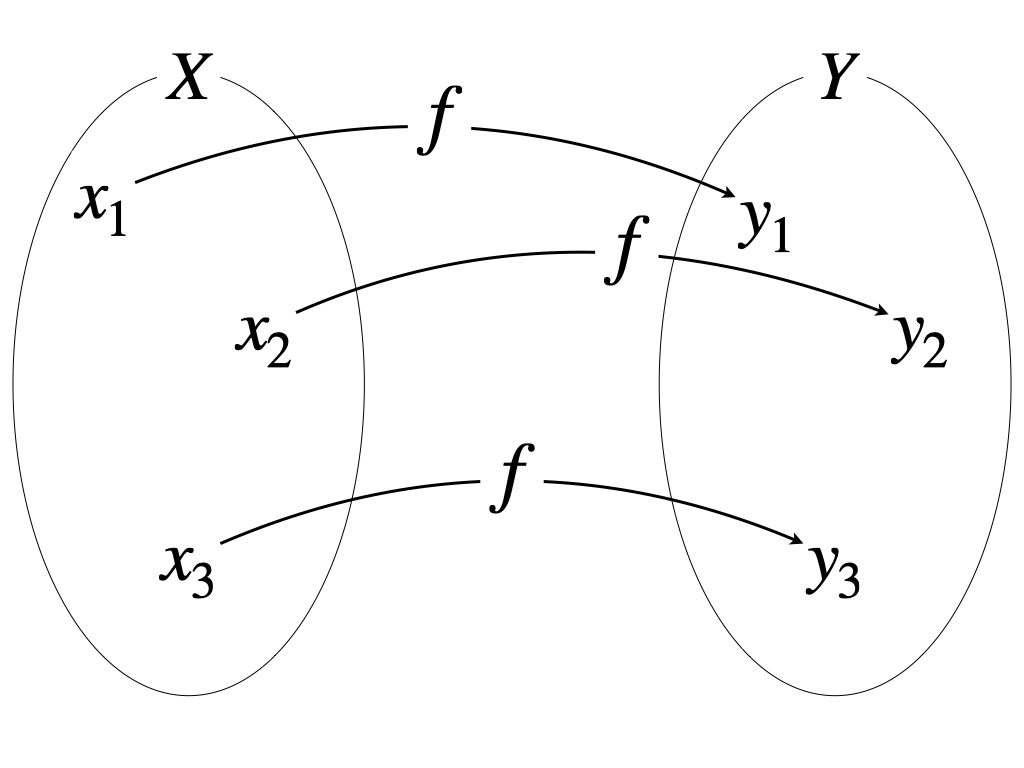
\includegraphics[width=5cm]{mapping/mapping1.png}
    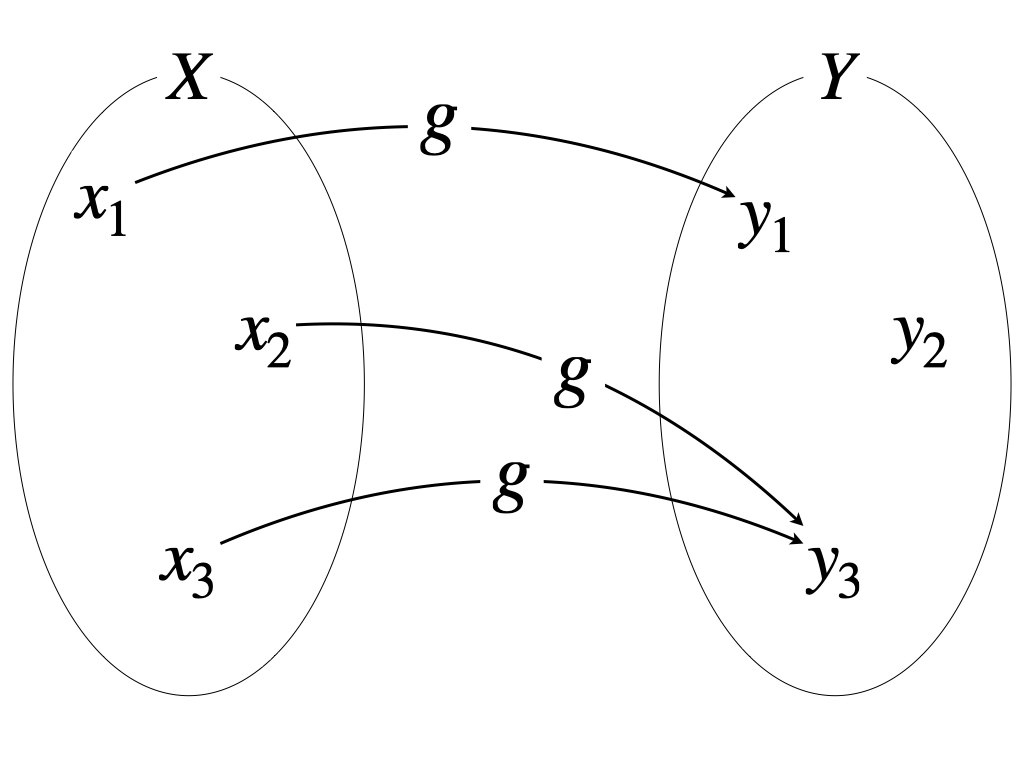
\includegraphics[width=5cm]{mapping/mapping2.png}
\end{center}

\begin{Definition}[全射, 単射]
    写像 $f\colon X \to Y$が
    \begin{itemize}
        \item 全射であるとは, 
        $\forall y\in Y\quad \exists x\in X\quad  y = f(x),$
        \item 単射であるとは, 
        $\forall x_1,x_2\in X\quad f(x_1) = f(x_2) \Rightarrow x_1 = x_2.$
    \end{itemize}
\end{Definition}

\begin{center}
    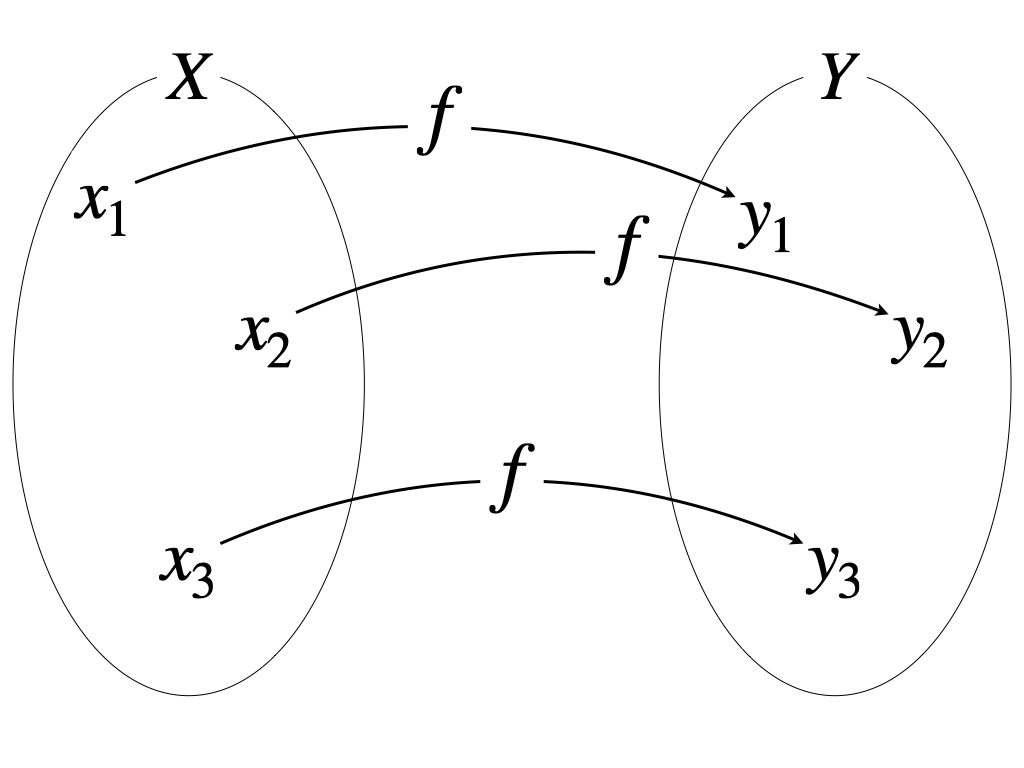
\includegraphics[width=5cm]{mapping/mapping1.png}
    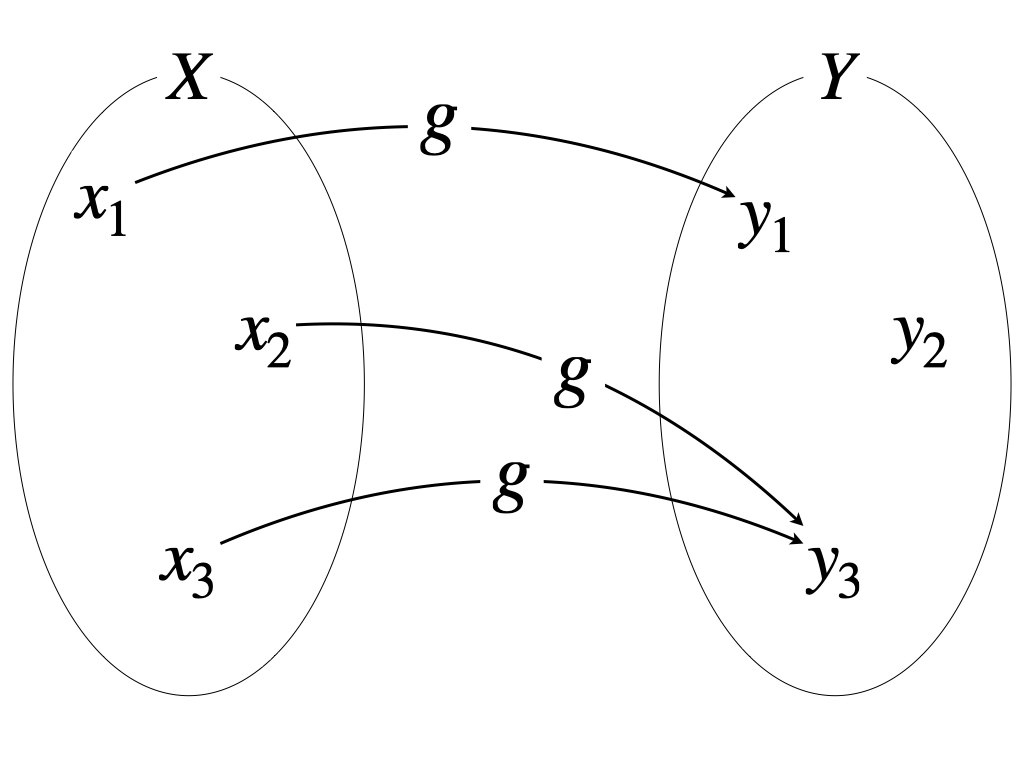
\includegraphics[width=5cm]{mapping/mapping2.png}
\end{center}



\subsection{置換}

$1,2,3$の入れ換え方を考える. 
$\sigma = \begin{pmatrix}
    1 & 2 & 3\\
    2 & 1 & 3
\end{pmatrix}$は, 
$1\mapsto 2,\quad 2\mapsto 1,\quad 3\mapsto 3$
という入れ換え方を表す. 
全パターンをあげると次の通り. 
\begin{align*}
    &\Big(\begin{array}{ccc}
        1 & 2 & 3 \\
        1 & 2 & 3 
    \end{array}\Big), 
    \Big(\begin{array}{ccc}
        1 & 2 & 3\\
        1 & 3 & 2
    \end{array}\Big), 
    \Big(\begin{array}{ccc}
        1 & 2 & 3\\
        2 & 1 & 3
    \end{array}\Big), \\
    &\Big(\begin{array}{ccc}
        1 & 2 & 3\\
        2 & 3 & 1
    \end{array}\Big), 
    \Big(\begin{array}{ccc}
        1 & 2 & 3\\
        3 & 1 & 2
    \end{array}\Big), 
    \Big(\begin{array}{ccc}
        1 & 2 & 3\\
        3 & 2 & 1
    \end{array}\Big)
\end{align*}

置換 $\sigma = \begin{pmatrix}
    1 & 2 & 3\\
    2 & 3 & 1
\end{pmatrix}$ を阿弥陀籤で表現できる. 
\begin{center}
    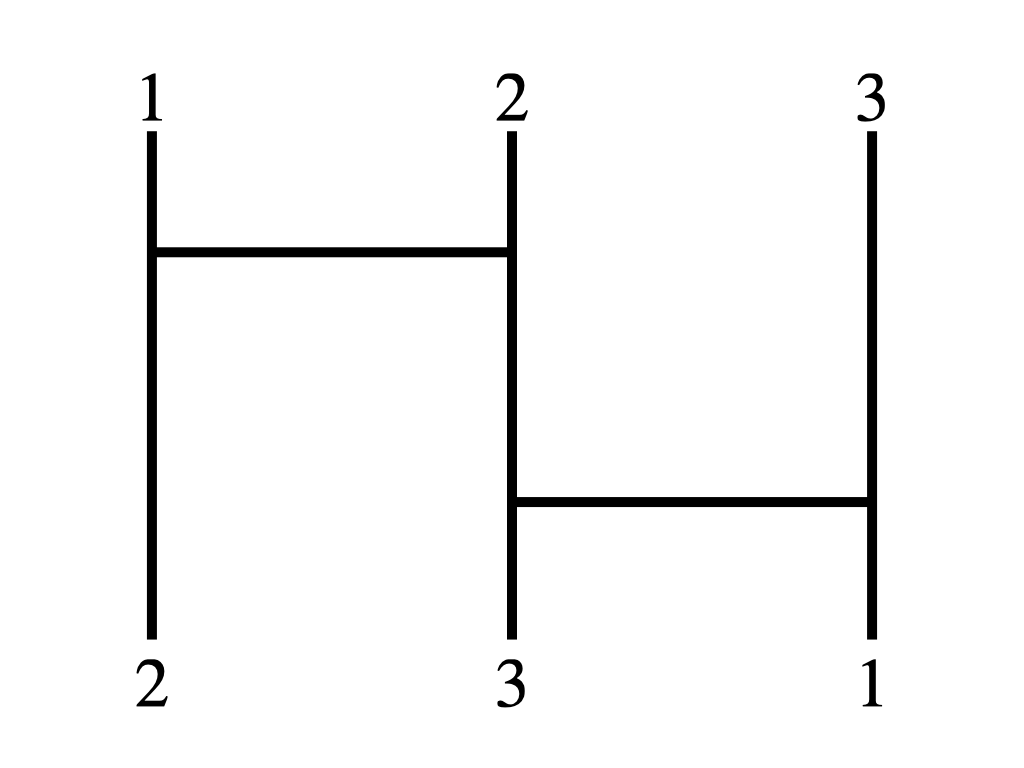
\includegraphics[width=5cm]{permutation/permutation1.png}
\end{center}


置換をつづけて行うことで別の置換になる. 
(阿弥陀籤を繋げて新しい籤を作る.)
\begin{align*}
    \begin{pmatrix}
        1 & 2 & 3\\
        2 & 1 & 3
    \end{pmatrix}
    \begin{pmatrix}
        1 & 2 & 3\\
        2 & 3 & 1
    \end{pmatrix}
    =
    \begin{pmatrix}
        1 & 2 & 3\\
        3 & 2 & 1
    \end{pmatrix}
\end{align*}
\begin{center}
    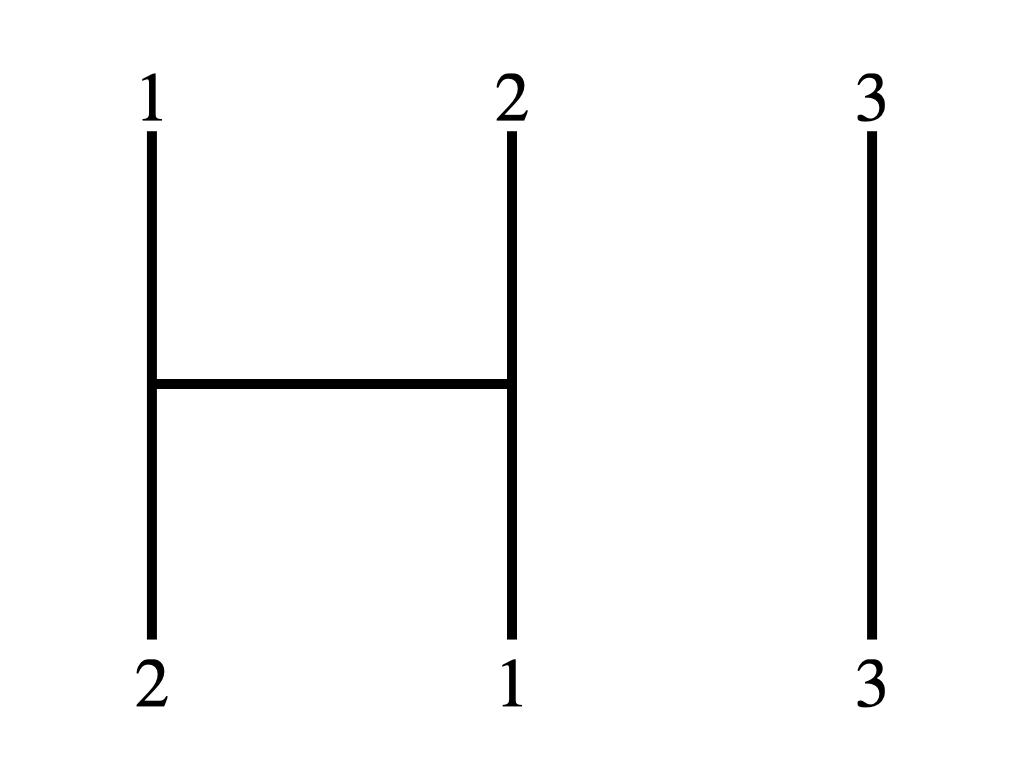
\includegraphics[width=4.3cm]{permutation/permutation2.png}
    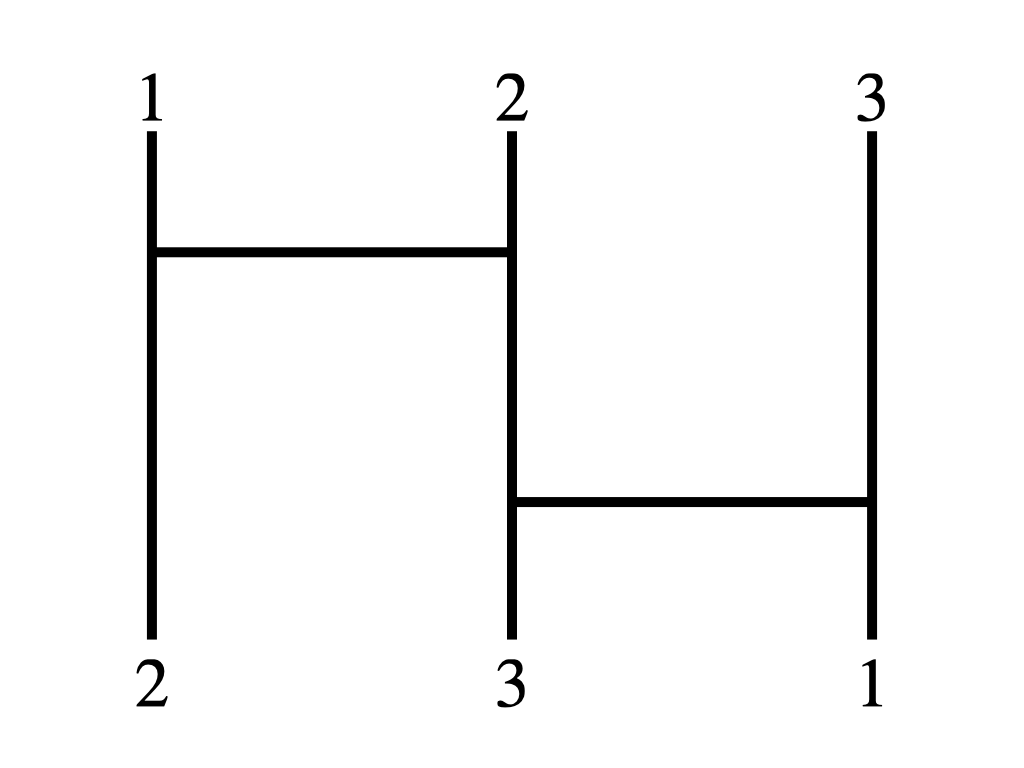
\includegraphics[width=4.3cm]{permutation/permutation1.png}
    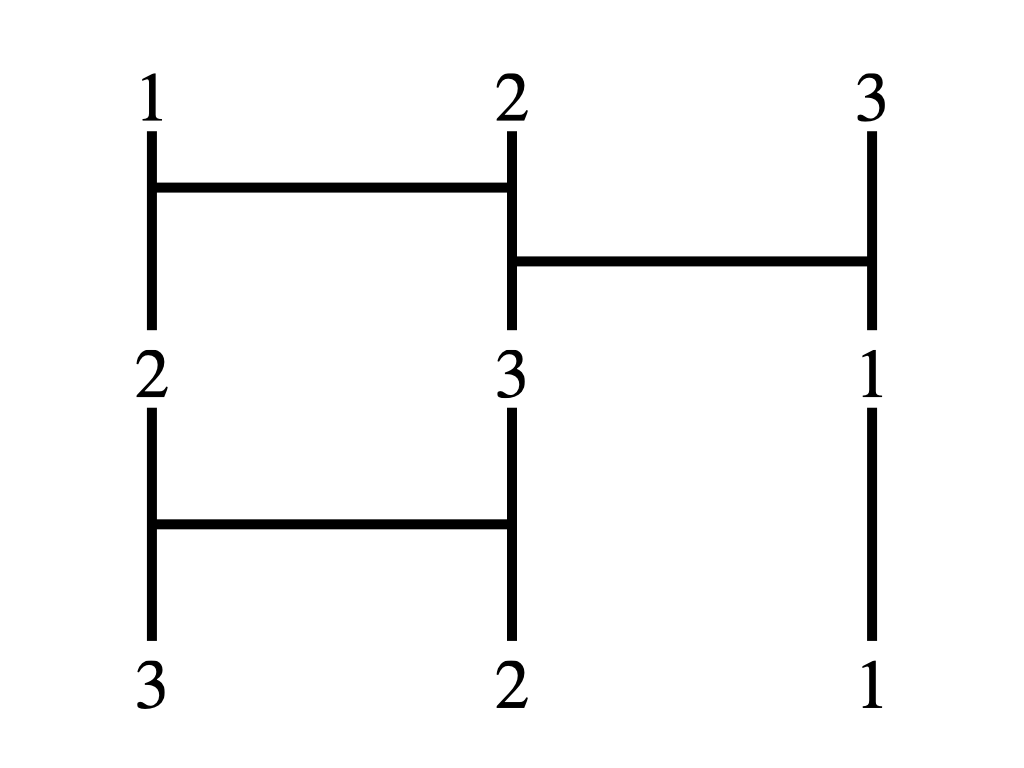
\includegraphics[width=4.3cm]{permutation/permutation3.png}
\end{center}

何もしない操作は, 水平橋ナシ. 
\begin{center}
    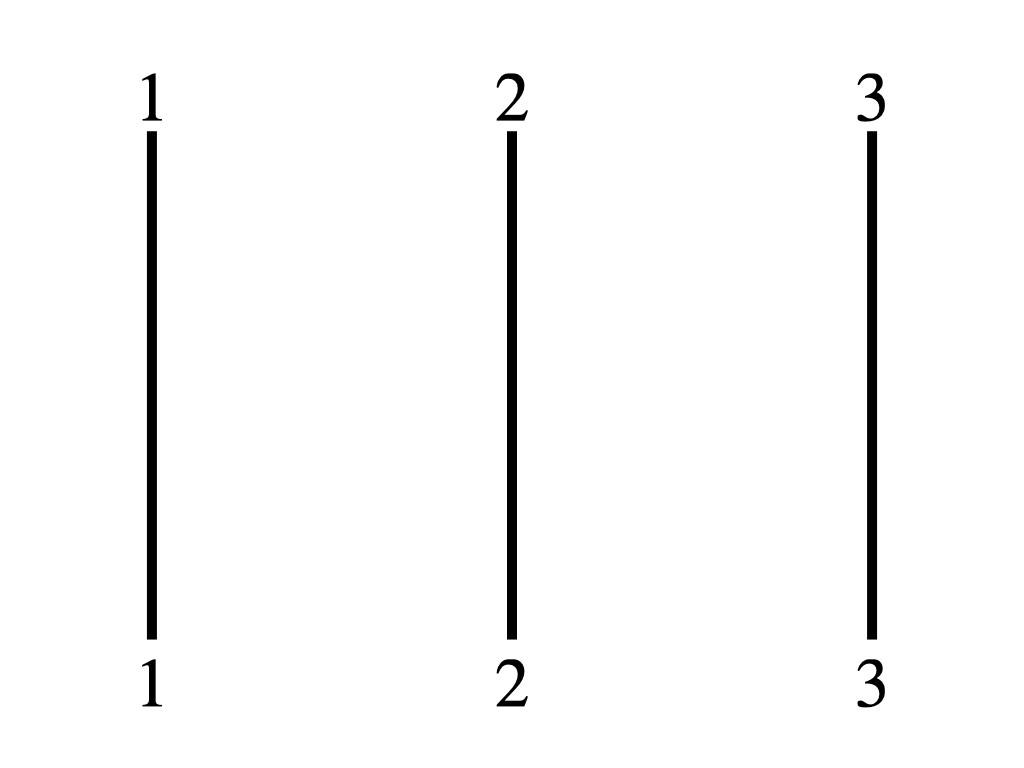
\includegraphics[width=5cm]{permutation/permutation6.png}
\end{center}

自分自身を逆さまにして繋げると元に戻る. 
\begin{align*}
    \begin{pmatrix}
        1 & 2 & 3\\
        2 & 3 & 1
    \end{pmatrix}
    \begin{pmatrix}
        1 & 2 & 3\\
        2 & 3 & 1
    \end{pmatrix}
    = 
    \begin{pmatrix}
        1 & 2 & 3\\
        1 & 2 & 3
    \end{pmatrix}
\end{align*}
\begin{center}
    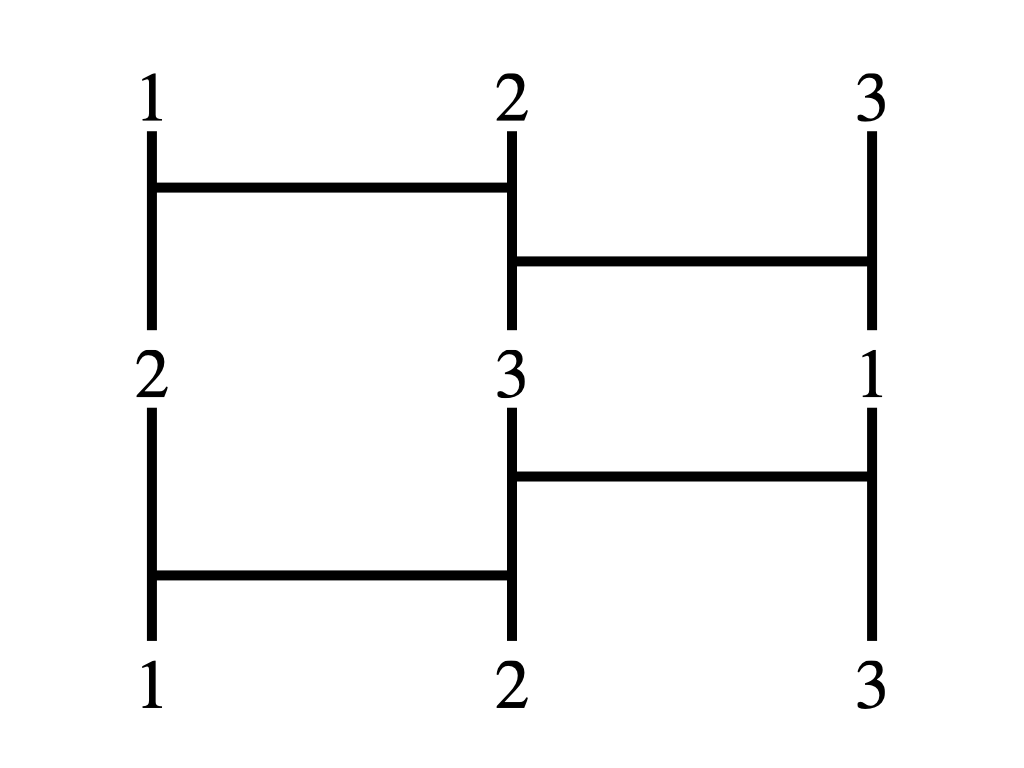
\includegraphics[width=6cm]{permutation/permutation5.png}
\end{center}

合成の順序によらず結果は同じ. 
\begin{center}
    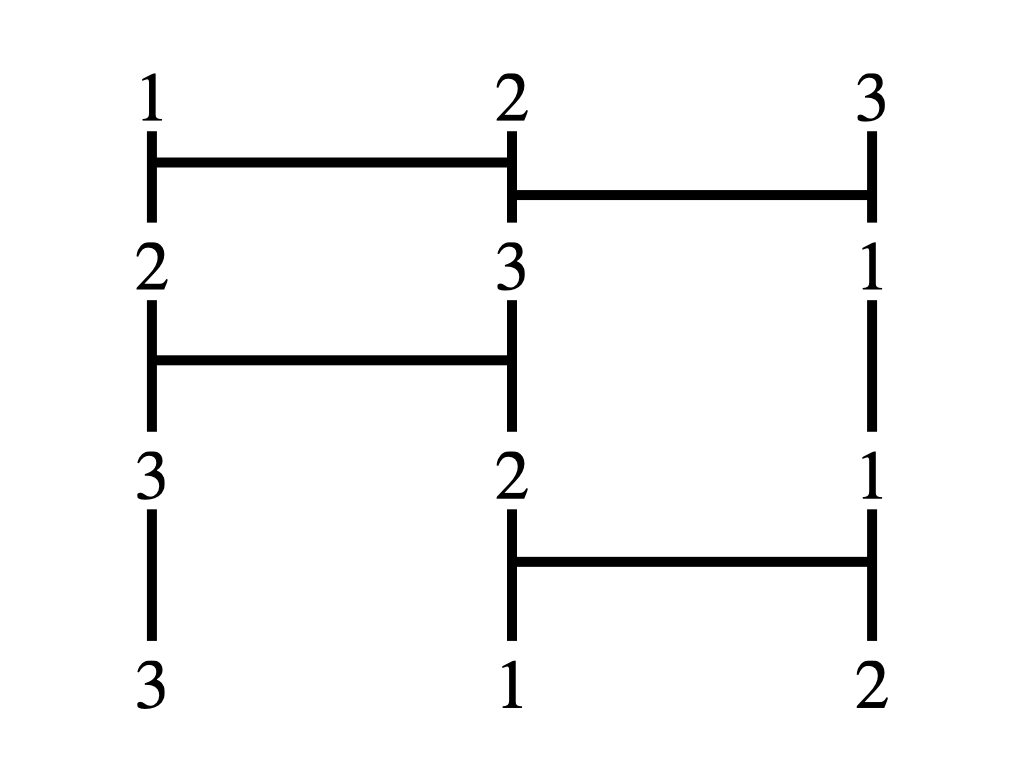
\includegraphics[width=6cm]{permutation/permutation7.png}
\end{center}

合成の順序によらず結果は同じ. 
\begin{align*}
    \begin{pmatrix}
        1 & 2 & 3\\
        1 & 3 & 2
    \end{pmatrix}
    \underbrace{
    \begin{pmatrix}
        1 & 2 & 3\\
        2 & 1 & 3
    \end{pmatrix}
    \begin{pmatrix}
        1 & 2 & 3\\
        2 & 3 & 1
    \end{pmatrix}
    }_{\text{先に計算}}
    &=
    \begin{pmatrix}
        1 & 2 & 3\\
        1 & 3 & 2
    \end{pmatrix}
    \begin{pmatrix}
        1 & 2 & 3\\
        3 & 2 & 1
    \end{pmatrix}\\
    &= 
    \begin{pmatrix}
        1 & 2 & 3\\
        3 & 1 & 2
    \end{pmatrix},
\end{align*}
\begin{align*}
    \underbrace{
    \begin{pmatrix}
        1 & 2 & 3\\
        1 & 3 & 2
    \end{pmatrix}
    \begin{pmatrix}
        1 & 2 & 3\\
        2 & 1 & 3
    \end{pmatrix}
    }_{\text{先に計算}}
    \begin{pmatrix}
        1 & 2 & 3\\
        2 & 3 & 1
    \end{pmatrix}
    &=
    \begin{pmatrix}
        1 & 2 & 3\\
        2 & 3 & 1
    \end{pmatrix}
    \begin{pmatrix}
        1 & 2 & 3\\
        2 & 3 & 1
    \end{pmatrix}\\
    &= 
    \begin{pmatrix}
        1 & 2 & 3\\
        3 & 1 & 2
    \end{pmatrix}.
\end{align*}

\subsection{置換のなす集合}

$1,2,\ldots,n$ の入れ換えを集めた集合を
$\mathfrak{S}_n$
で表す.

置換の個数は $1,\ldots,n$の並べ方の個数と同じ. 
つまり, 
\begin{align*}
    |\mathfrak{S}_n| 
    = \left|\left\{ 
        \sigma = \Big(\begin{array}{ccc}
        1 & \cdots & n \\
        \sigma(1) & \cdots & \sigma(n)
    \end{array}\Big) 
    \right\}\right| = n!
\end{align*}

例を見てみる.
$n=1$のとき,$1\mapsto 1$のひとつだけ.
    
$n=2$のとき,
\begin{align*}
    \Big(\begin{array}{cc}
        1 & 2 \\
        1 & 2 
    \end{array}\Big),
    \Big(\begin{array}{cc}
        1 & 2 \\
        2 & 1 
    \end{array}\Big) 
\end{align*}
の2コ.

$n=3$のとき,さっきやった6コ.

$n=4$のとき,次の24コ.
\begin{align*}
    &\Big(\begin{array}{cccc}
        1 & 2 & 3 & 4 \\
        1 & 2 & 3 & 4
    \end{array}\Big), 
    \Big(\begin{array}{cccc}
        1 & 2 & 3 & 4 \\
        1 & 2 & 4 & 3
    \end{array}\Big),
    \Big(\begin{array}{cccc}
        1 & 2 & 3 & 4 \\
        1 & 3 & 2 & 4
    \end{array}\Big), 
    \Big(\begin{array}{cccc}
        1 & 2 & 3 & 4 \\
        1 & 3 & 4 & 2
    \end{array}\Big),\\%=======================
    &\Big(\begin{array}{cccc}
        1 & 2 & 3 & 4 \\
        1 & 4 & 2 & 3
    \end{array}\Big),
    \Big(\begin{array}{cccc}
        1 & 2 & 3 & 4 \\
        1 & 4 & 3 & 2
    \end{array}\Big), 
    \Big(\begin{array}{cccc}
        1 & 2 & 3 & 4 \\
        2 & 1 & 3 & 4
    \end{array}\Big), 
    \Big(\begin{array}{cccc}
        1 & 2 & 3 & 4 \\
        2 & 1 & 4 & 3
    \end{array}\Big), \\%=======================
    &\Big(\begin{array}{cccc}
        1 & 2 & 3 & 4 \\
        2 & 3 & 1 & 4
    \end{array}\Big), 
    \Big(\begin{array}{cccc}
        1 & 2 & 3 & 4 \\
        2 & 3 & 4 & 1
    \end{array}\Big), 
    \Big(\begin{array}{cccc}
        1 & 2 & 3 & 4 \\
        2 & 4 & 1 & 3
    \end{array}\Big),
    \Big(\begin{array}{cccc}
        1 & 2 & 3 & 4 \\
        2 & 4 & 3 & 1
    \end{array}\Big), \\%========================
    &\Big(\begin{array}{cccc}
        1 & 2 & 3 & 4 \\
        3 & 1 & 2 & 4
    \end{array}\Big),  
    \Big(\begin{array}{cccc}
        1 & 2 & 3 & 4 \\
        3 & 1 & 4 & 2
    \end{array}\Big), 
    \Big(\begin{array}{cccc}
        1 & 2 & 3 & 4 \\
        3 & 2 & 1 & 4
    \end{array}\Big),   
    \Big(\begin{array}{cccc}
        1 & 2 & 3 & 4 \\
        3 & 2 & 4 & 1
    \end{array}\Big), \\%=========================
    &\Big(\begin{array}{cccc}
        1 & 2 & 3 & 4 \\
        3 & 4 & 1 & 2
    \end{array}\Big),
    \Big(\begin{array}{cccc}
        1 & 2 & 3 & 4 \\
        3 & 4 & 2 & 1
    \end{array}\Big), 
    \Big(\begin{array}{cccc}
        1 & 2 & 3 & 4 \\
        4 & 1 & 2 & 3
    \end{array}\Big), 
    \Big(\begin{array}{cccc}
        1 & 2 & 3 & 4 \\
        4 & 1 & 3 & 2
    \end{array}\Big), \\%=========================
    &\Big(\begin{array}{cccc}
        1 & 2 & 3 & 4 \\
        4 & 2 & 1 & 3
    \end{array}\Big), 
    \Big(\begin{array}{cccc}
        1 & 2 & 3 & 4 \\
        4 & 2 & 3 & 1
    \end{array}\Big), 
    \Big(\begin{array}{cccc}
        1 & 2 & 3 & 4 \\
        4 & 3 & 1 & 2
    \end{array}\Big), 
    \Big(\begin{array}{cccc}
        1 & 2 & 3 & 4 \\
        4 & 3 & 2 & 1
    \end{array}\Big) 
\end{align*}

$X\to Y$ という写像を集めて集合を作ってみる. 
\begin{align*}
    \Map(X,Y)\coloneqq \{\text{写像} X\to Y \}
\end{align*}
$f\in \Map(X,Y)$ とは$f\colon X \to Y$ ということ. 
写像に条件をつけたものの集合も考えられる. 
\begin{align*}
    \End(X)&\coloneqq \Map(X,X), \\
    \Aut(X)&\coloneqq \{f \in \End(X); \text{$f$は全単射}\}
\end{align*}
$[n] = \{1,\ldots,n\}$とかくことにすると, 
$\mathfrak{S}_n = \Aut([n])$ということになる. 

$\Aut(X)$の元 (つまり全単射像) 
$f,g,h\in \Aut(X)$は次の性質を持っている. 
\begin{itemize}
    \item $h\circ (g\circ f) = (h\circ g)\circ f$
    \item $\id_X \circ f = f \circ \id_X = f$
    \item $f^{-1}\circ f = f^{-1} \circ f = \id_X$
\end{itemize}
これらの性質を満たす集合を群 (group) という. 
$\mathfrak{S_n}$の元, すなわち置換はこれらの性質を満たしていた. 
$\mathfrak{S_n}$には 対称群 という名前が付いている. 


\subsection{置換の行列表現}

置換 $\sigma = \begin{pmatrix}
    1 & 2 & 3\\
    3 & 1 & 2
\end{pmatrix}$に対し, 
ベクトル 
$x = 
\begin{pmatrix}
    x_1\\x_2\\x_3
\end{pmatrix}$
を, 第$i$成分を第$\sigma(i)$成分に移動させたベクトル
$\begin{pmatrix}
    x_2\\x_3\\x_1    
\end{pmatrix}$
に対応させる行列を$A_\sigma$とする. 

\begin{align*}
    \begin{pmatrix}
        x_2\\x_3\\x_1    
    \end{pmatrix} = A_\sigma \begin{pmatrix}
        x_1\\x_2\\x_3    
    \end{pmatrix}
\end{align*}
から, $A_\sigma$の成分を求めてみると, 
\begin{align*}
    A_\sigma = 
    \begin{pmatrix}
        0 & 1 & 0 \\
        0 & 0 & 1 \\
        1 & 0 & 0
    \end{pmatrix}
\end{align*}
となる. 

行列は
\begin{align*}
    A(x+y) = Ax + Ay, \quad A(cx) = cAx
\end{align*}
という性質を持っていた. 

写像でこの性質を満たすものを線形写像といって, 
$n$次元ベクトルから自分自身への全単射な線形写像の集合を 
$GL_n(\mathbf{R})$とかくと, 
これは, 正則な$n\times n$行列の集合と思える. 

さっきやった `置換$\longleftrightarrow$ 行列' の対応は
$\mathfrak{S}_n \to GL_n(\mathbf{R})$
という写像になっている. (置換の行列表現という.)

\section{数研の活動について}
\subsection*{通年の活動}

\subsubsection*{セミナー}
主な活動は少人数でのセミナーである. 
2・3人の発表者とチューターで行うという
パターンが多いが, 編成は自由である. 
1セメスターで区切ることが多いと思うが, 
各メンバーの希望に応じて, 
1年以上行ったりすることもある. 

\subsubsection*{例会}
おおよそ月に一回のペースで部員全員で集まる. 
%内容が多くなるので詳細は後述する. 
%なお, 
%2020年度はコロナウイルス感染を
%防ぐためキャンパス入構が制限されていた. そのため例会はほとんど行えず, 活動も滞っていた. (zoom などリモート会議ツールを用いてのリモート例会を行うなど, 工夫の余地はあったと思う. この点は2020年度の反省点である.)


\subsubsection*{新歓方程}
1年生向けに数学の解説を執筆し
ブースに置いておく. 
%大体, 2・3コくらいの記事があれば十分だと思う. 
%ちなみに, 2020年度はブース出展そのものが
%中止となったので配布しなかった. 
%その代わりに, 2019年度の方程の
%PDF データを数理科slackの
%数研チャンネルにて共有した. 
2019年度は
\begin{itemize}
    \item 実数の完備性
    \item 常微分方程式の解法
\end{itemize}
のような記事があったと思う. 
(筆者の記憶によるので曖昧. )

\subsection*{4-5月 --- 新歓講演}

1年生向けに, 会員 (主に2年生) が自由な話題で
講演する. 
大体2人くらいがそれぞれ1コマ (90分) の枠で
話すパターンが多いと思う. 
このとき, 60分くらいで話し終えて, 
15分くらいを質疑応答に充てるイメージ. 

2019年度は, 4月11, 17日に60分ずつ教室を借りて行った. 
2020年度は, 5月26, 28日に一コマずつzoomで行った. 
告知については, 一年生向けの授業にて担当教員を通して
行ったり, サブゼミ・slack・line を用いて行った. 

過去の講演内容には, 以下のようなものがある. 
\begin{itemize}
    \item 自然数, ペアノの公理など (2020年度) 
    \item 実数の連続性 (2020年度) 
    \item 代数学と物理学 (2019年度) 
    \item 応用数学への入門 (2019年度)
    \item 数理論理学 (2018年度)
\end{itemize}

\subsection*{8-9月 --- 夏期合宿}

2泊3日か3泊4日くらいで合宿をする.
2020年度以降は実施していない.

\subsection*{10-12月 --- 機関紙作成}

その年度に勉強したことについて自分の言葉でまとめる.

\subsection*{2-3月 --- 春季合宿}

2泊3日か3泊4日くらいで合宿をする.
2020年度以降は実施していない.



\begin{thebibliography}{15}
    \bibitem{saito1} 斎藤毅, 微積分, 東京大学出版会, 2013.\\
    \ref{sec-cal}章の参考書.
    \bibitem{satake1} 佐武一郎, 線形代数学 (新装版), 裳華房, 2015.\\
    \ref{sec-la}章の参考書.
    \bibitem{sato1} 佐藤文広, 数学ビギナーズマニュアル [第2版], 日本評論社, 2014.\\
    数学の方言?に詳しい.
    \bibitem{take1} 竹山美宏, 数学書の読みかた, 森北出版, 2022.\\
    最近出た本.きちんと目は通してないが,推し数学者の本なので挙げておく.
\end{thebibliography}

\end{document}